\documentclass[12pt,letterpaper]{article}

\usepackage{fullpage}
\usepackage{hyperref}
\usepackage{amsmath}
\usepackage{graphicx}
\usepackage{tikz}
\usepackage{float}
\usepackage{subcaption}
\usepackage{hyperref}

\usetikzlibrary{arrows}

\begin{document}

\begin{flushright}
Kyle Cesare \\
Kevin Hess \\
Bryce Holley
\end{flushright}

{\Large\center\textbf{Programming Assignment 3: TSP} \\}

\section{Algorithm}
Our algorithm is a composite of two algorithms: nearest neighbor and 2-opt. We
use a greedy algorithm to produce an initial guess to pass to a heuristic
algorithm, which iteratively improves upon that guess. We decided on this method
with the idea that our program might not be able to finish given a time
constraint. By implementing an improvement heuristic, we ensure that we would
have a valid solution even if the optimization was not fully computed.

\subsection{Nearest Neighbor}
Nearest neighbor is a greedy algorithm which works on the idea that connecting
each vertex in a vertex set to its closest possible neighbor produces a
reasonably short tour. The algorithm starts by selecting the first node from the
original set of cities and then calculating the distance to each of the other
nodes. The closest possible node is selected next. The distances are then
calculated from this new node, excluding the distance to the original node which
was already traversed. Each node is added to the tour in this manner until every
node in the original vertex set has been added to the tour.

\subsection{2-opt}
Given a tour, the 2-opt algorithm finds two edges within the tour that cross
over each other, and rearranges the tour so that they no longer cross. That is,
for a tour $T$, if there are two edges $(V_{i-1}, V_i)$ and $(V_j, V_{j+1})$
which intersect, the algorithm reverses vertices $\{V_i, \ldots, V_j\}$ in the
tour. The resulting tour, $T'$, has the same beginning and end but the crossed
subset is reversed, and is thus uncrossed. This operation is repeated until no
more improvements can be made in this manner.


\begin{figure}[H]
  \centering
  \caption{A tour before and after applying 2-opt.}
  \begin{minipage}{.2\textwidth}
    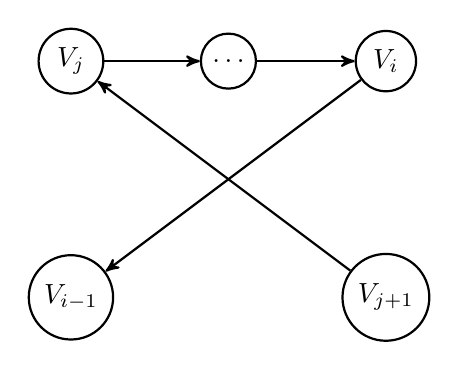
\begin{tikzpicture}[->,>=stealth',thick]
      % With cross
        % Start/end nodes
        \node[draw, circle] (a) at (2, 0) {$V_{i-1}$};
        \node[draw, circle] (b) at (6, 0) {$V_{j+1}$};

        % Path
        \node[draw, circle] (s0) at (2, 3) {$V_j$};
        \node[draw, circle] (s1) at (4, 3) {$\ldots$};
        \node[draw, circle] (s2) at (6, 3) {$V_i$};

        \draw [->] (b) -- (s0);
        \draw [->] (s0) -- (s1);
        \draw [->] (s1) -- (s2);
        \draw [->] (s2) -- (a);

    \end{tikzpicture}
  \end{minipage}
  \hspace{1.5in}
  \begin{minipage}{.2\textwidth}
    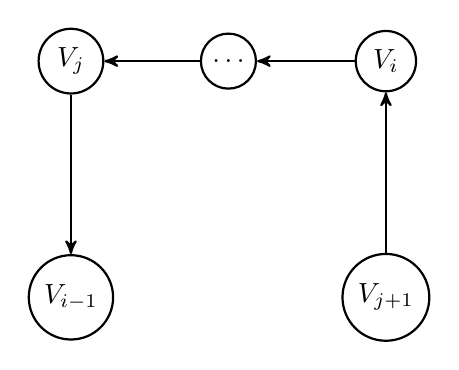
\begin{tikzpicture}[->,>=stealth',thick]
      % Without cross
        % Start/end nodes
        \node[draw, circle] (a) at (2, 0) {$V_{i-1}$};
        \node[draw, circle] (b) at (6, 0) {$V_{j+1}$};

        % Path
        \node[draw, circle] (s0) at (2, 3) {$V_j$};
        \node[draw, circle] (s1) at (4, 3) {$\ldots$};
        \node[draw, circle] (s2) at (6, 3) {$V_i$};

        \draw [->] (s0) -- (a);
        \draw [->] (b) -- (s2);
        \draw [->] (s1) -- (s0);
        \draw [->] (s2) -- (s1);

    \end{tikzpicture}
  \end{minipage}
\end{figure}

Our implementation of 2-opt utilizes two for-loops to compare all pairs of edges
for possible improvements. These loops are nested in a while block so that the
entire process restarts every time an improvement is made until no more
improvements can be made.

\section{Implementation}

We implemented our algorithm in Python using NumPy. We build our nearest
neighbor approximation by moving nodes from a vertex set $V$ to our tour $U$.
For each node, we recalculate the distance to every other node and choose the
smallest.

We then pass our initial tour into our 2-opt iterative algorithm. Here, we
iterate over every pair of edges in the tour. We check if reversing the
intermediate vertices produces a better tour. If it does, we mark the modified
tour as our current best and restart the 2-opt process. For improved
performance, we do not rebuild the entire modified tour until we know it is
actually better than the current best. We are able to calculate its length in
$O(1)$ time, rather than having to reiterate the entire tour.

Unfortunately, we were not able to run the 2-opt algorithm to completion in the
given time. We could further improve upon our solution by rewriting our program
in a faster language like C or C++. Such an implementation would hopefully be
able to complete the entire iterative process in the given time.

\section{References}
\begin{enumerate}
  \item \url{https://en.wikipedia.org/wiki/Local_search_(optimization)}
  \item \url{http://www.seas.gwu.edu/~simhaweb/champalg/tsp/tsp.html}
  \item \url{https://cstheory.stackexchange.com/questions/9241/approximation-algorithms-for-metric-tsp}
\end{enumerate}

\end{document}
